\documentclass[../ewet_cwc_report.tex]{subfiles}

\begin{document}
\section{Design Objectives and Components}

\noindent
The objective of our turbine design team was to create a
turbine that performed well in the CWC test environment. The
turbine had to fit within the bounding box shown in
Figure \ref{img:constraints}. The bounding box is a
\qty{45}{\cm} cube mounted on a \qty{15}{\cm} diameter cylinder
which extends downwards to the underwater foundation attachment
resting on the $24 \times 25 \times 15$ cube of water immersed
in sand.  The turbine blades needed to be completely enclosed
in the cube. The turbine was supposed to start at the lowest
wind speed possible, then produce power of varying levels until
wind speeds of \qty{11}{\m\per\s} and respond to load
disconnect scenario in a controlled manner.  All turbine
components were to be designed to withstand wind speeds of
\qty{22}{\m\per\s}. The electrical system needed to work with
an out of box motor to be used as a generator. The motor
produced AC power which needed to be converted to usable DC
power. A system to adjust resistance on the circuit to maintain
optimal power output during the variable conditions needed to
be designed. Finally, a control system needed to be designed to
adjust pitch based on rotational speed of the turbine and
maintain maximum torque generated from the wind.

\begin{figure}[th]
  \centering
  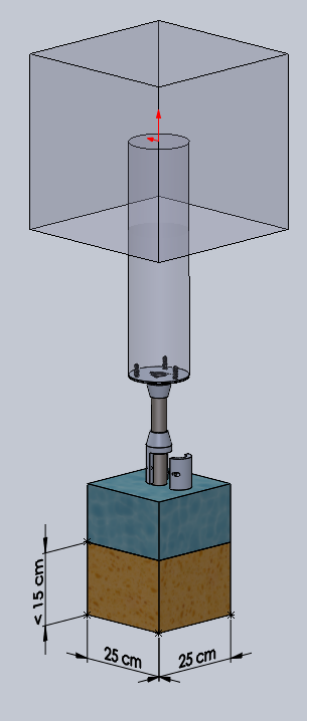
\includegraphics[width=0.2\textwidth]{../_images/design_constraints.png}
  \caption{Design constraints}
  \label{img:constraints}
\end{figure}

\end{document}
